% Source: graduate-coursework/Prior_Semesters/Sp24/EMCH354/assignments/HW2/HW2.tex

\documentclass[border=4pt]{standalone}
\usepackage{amsmath}
\usepackage{tikz}
\usetikzlibrary{patterns}
\usetikzlibrary{arrows.meta, decorations.pathmorphing}

\definecolor{bluecolor}{RGB}{173,216,230}
\definecolor{purplecolor}{RGB}{210,180,222}
\definecolor{pinkcolor}{RGB}{255,182,193}
\definecolor{orangecolor}{RGB}{252, 213, 180}

\begin{document}
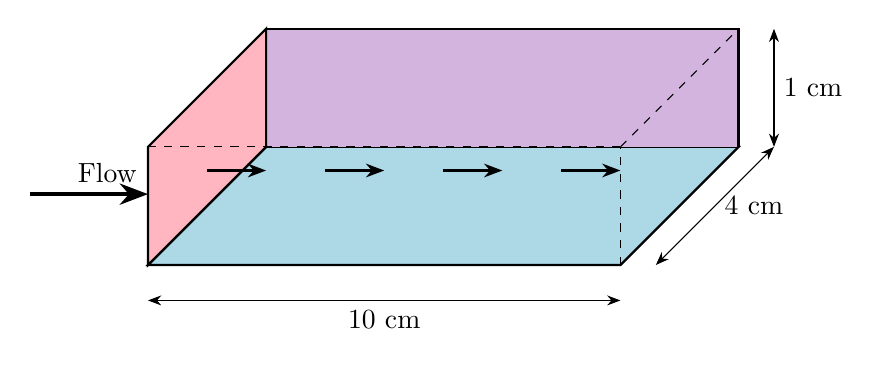
\begin{tikzpicture}[scale=1.5, >=Stealth]
    % Top side of the duct
    \fill[bluecolor] (0,0) -- (4,0) -- (5,1) -- (1,1) -- cycle;
    \draw[thick] (0,0) -- (4,0) -- (5,1) -- (1,1) -- cycle;
    
    % Side of the duct
    \fill[purplecolor] (5,1) -- (5,2) -- (1,2) -- (1,1) -- cycle;
    \draw[thick] (5,1) -- (5,2) -- (1,2) -- (1,1);
    
    % Front of the duct (visible part)
    \fill[pinkcolor] (0,0) -- (1,1) -- (1,2) -- (0,1) -- cycle;
    \draw[thick] (0,0) -- (1,1) -- (1,2) -- (0,1) -- cycle;
    
    % Dashed lines for the wireframe view
    \draw[dashed] (4,0) -- (4,1);
    \draw[dashed] (4,1) -- (4,1,-2.5);
    \draw[dashed] (4,1) -- (0,1);
    
    % Flow arrows on top side
    \foreach \x in {0.5,1.5,...,3.5}
        \draw[->,thick] (\x,0.8) -- ++(0.5,0);
    
    % Labeling the duct dimensions
    \draw[<->] (0,-0.3) -- node[below] {10 cm} (4,-0.3); % Length
        % Labeling the back
    \draw[<->] (4.3,0) -- node[right] {4 cm} (5.3,1); % Width
    \draw[<->] (5.3,1) -- node[right] {1 cm} (5.3,2); % Height

    % Labeling the flow
    \draw[->,ultra thick] (-1,0.6) -- (0,0.6) node[above left] {Flow};
\end{tikzpicture}
\end{document}
